
% Let us try to further condense the 'minimal lectures'.

\documentclass[12pt, a4paper]{article}

\raggedbottom

\RequirePackage[l2tabu, orthodox]{nag}

\usepackage[top=20mm,bottom=20mm,left=25mm,right=25mm]{geometry}

% \usepackage{showkeys}

\usepackage{amsfonts, amsmath}

\usepackage{pgf}
\usepackage{tikz}

\usepackage{multirow}

\usepackage{pgf}
\usepackage{tikz}

\usepackage{amsthm}
\newtheoremstyle{break}{9pt}{9pt}{\itshape}{}{\bfseries}{}{\newline}{}
\theoremstyle{break}    
\newtheorem{exo}{Exercise}
\newtheorem{hyp}[exo]{Axiom}
\newtheorem{res}[exo]{Result}
\newtheorem{defn}[exo]{Definition}

\usepackage[colorlinks=true,linktoc=all,linkcolor=black,citecolor=red,urlcolor=blue]{hyperref}

\title{\bfseries A crash course on two-dimensional \\ conformal field theory}

\author{Sylvain Ribault \vspace{2mm}
\\
{\normalsize CEA Saclay, Institut de Physique Th\'eorique}
 \\
 {\footnotesize \ttfamily sylvain.ribault@ipht.fr }
}

\begin{document}


\maketitle


\begin{abstract}
We provide a brief but self-contained introduction to conformal field theory on the Riemann sphere. We first introduce general axioms such as local conformal invariance, and derive Ward identities and BPZ equations. We then define Liouville theory by specific axioms on its spectrum and degenerate fields. We solve the theory and study its four-point functions.
\end{abstract}

\tableofcontents

\clearpage

\hypersetup{linkcolor=blue}

%\numberwithin{equation}{section}


This text was written with brevity as the main concern, so as to be the basis for about 100 minutes' worth of lectures. For more details, see the longer lecture notes \cite{rib16} and the full review article \cite{rib14}.

\section{Conformal field theory}

\subsection{The Virasoro algebra and its representations}

By definition, conformal transformations are transformations that preserve angles. 
In two dimensions with a complex coordinate $z$, any holomorphic map preserves angles.
Infinitesimal conformal transformations are
\begin{align}
 z \mapsto z + \epsilon z^{n+1}\qquad (n\in\mathbb{Z}\ , \ \epsilon\ll 1) \ .
\end{align}
These transformations act on functions of $z$ via the differential operators 
\begin{align}
 \ell_n = -z^{n+1}\frac{\partial}{\partial z}\ ,
\end{align}
and these operators generate the Witt algebra, with commutation relations
\begin{align}
 [\ell_n,\ell_m ] = (n-m)\ell_{m+n}\ .
\end{align}
In a quantum theory, symmetry transformations act projectively on states. 
Projective representations of an algebra are equivalent to representations of a centrally extended algebra. 

\begin{defn}[Virasoro algebra]
 ~\label{def:vir}
 The central extension of the Witt algebra is called the Virasoro algebra. It has the generators $(L_n)_{n\in\mathbb{Z}}$ and $\mathbf 1$, and the commutation relations
 \begin{align}
  [\mathbf 1, L_n] = 0 \quad , \quad [L_n,L_m] = (n-m)L_{n+m} +\frac{c}{12}(n-1)n(n+1)\delta_{n+m,0}\mathbf 1 \ ,
  \label{eq:vir}
 \end{align}
 where the number $c$ is called the central charge. 
\end{defn}

The spectrum, i.e. the space of states, must be a representation of the Virasoro algebra.
We want to interpret $L_0$ as the energy operator, so its eigenvalues, called conformal dimensions, must be bounded from below. But 
\begin{align}
 L_0 |v\rangle = \Delta |v\rangle  \qquad \Rightarrow \qquad L_0 L_n|v\rangle =  (\Delta-n)L_n|v\rangle \ .
\end{align}
So $L_{n>0}$ decrease conformal dimensions, and must therefore kill the state with the lowest dimension. 

\begin{defn}[Primary and descendent states, level, Verma module]
 ~\label{def:prim}
 A primary state with conformal dimension $\Delta$ is a state $|v\rangle$ such that 
 \begin{align}
  L_0 |v\rangle = \Delta |v\rangle \quad , \quad L_{n>0} |v\rangle = 0\ .
 \end{align}
A descendent of $|v\rangle$ is a linear combination of states of the type $|w\rangle = \prod_{i=1}^k L_{-n_i} |v\rangle$ with $0<n_i$. 
The level of such a state is the positive integer $N=\sum_{i=1}^k n_i$ such that $L_0|w\rangle = (\Delta + N)|w\rangle$. The Verma module $\mathcal V_\Delta$ is the representation whose basis is made of the states $|w\rangle = \prod_{i=1}^k L_{-n_i} |v\rangle$ with $k\geq 0$ and $0<n_1\leq n_2 \leq \dots \leq n_k$.
\end{defn}
Let us plot a basis of a Verma module up to the level $N=2$:
\begin{align}
 \begin{tikzpicture}[scale = .25, baseline=(current  bounding  box.center)]
  \draw[-latex, very thick] (20, 0) -- (20, -14) node [right] {$N$};
  \foreach \x in {0, ..., 2}
  {
  \draw [dotted] (-20, {-6*\x}) -- (20, {-6*\x}) node [right] {${\x}$};
  }
  \node[fill = white] at (0, 0) (0) {$|v\rangle$};
  \node[fill = white] at (-4,-6) (1) {$L_{-1}|v\rangle$};
  \node[fill = white] at (-8, -12) (11) {$L_{-1}^2|v\rangle$};
  \node[fill = white] at (4,-12) (2) {$L_{-2}|v\rangle$};
  \draw[-latex] (0) -- (1);
  \draw[-latex] (1) -- (11);
  \draw[-latex] (0) -- (2);
 \end{tikzpicture}
\end{align}
If a Verma module is not irreducible, i.e. if it has a nontrivial submodule, then the state with the lowest conformal dimension in that submodule must again be a primary state, while also being a descendent state.

\begin{defn}[Null vectors]
 ~\label{def:nv}
 A descendent state that is also primary is called a null vector or singular vector.
\end{defn}

In the Verma module $\mathcal V_\Delta$, let us find out whether $L_{-1}|v\rangle$ is a null vector:
\begin{align}
L_n L_{-1}|v\rangle \underset{n\geq 1}{=} [L_n, L_{-1}] |v\rangle = (n+1) L_{n-1}|v\rangle = 
\left\{\begin{array}{ll} 0 &  \quad \text{if } n\geq 2 \\ 2\Delta |v\rangle & \quad \text{if } n = 1 \end{array}\right. 
\end{align}
So $L_{-1}|v\rangle$ is a null vector if and only if $\Delta=0$, and the Verma module $\mathcal V_0$ is reducible.
Let us now look for null vectors at the level $N=2$. Let $|\chi\rangle = (L_{-1}^2 + a L_{-2})|v\rangle$, then $L_{n\geq 3} |\chi \rangle =0$ and 
 \begin{align}
  L_1 |\chi\rangle = \left((4\Delta+2) + 3a\right) L_{-1}|v\rangle
  \quad , \quad L_2 |\chi\rangle= \left(6\Delta + (4\Delta +\tfrac12 c)a\right) |v\rangle\ .
 \end{align}
 There exists a value of $a$ such that $L_1|\chi\rangle = L_2|\chi\rangle =0$ if and only if 
 \begin{align}
 \Delta = \frac{1}{16}\left( 5-c\pm\sqrt{(c-1)(c-25)} \right) \ .
 \label{eq:dpm}
\end{align}
In order to simplify this formula, let us introduce other notations for $c$ and $\Delta$. We define
\begin{align}
 \text{the background charge } Q \ , & \quad c = 1+6Q^2\ , \quad \text{up to } Q \to -Q\ ,
 \\
 \text{the coupling constant } b \ , & \quad Q = b+\frac{1}{b} \ , \quad \text{up to } b\to \pm b^{\pm 1}\ ,
 \\
 \text{the momentum } \alpha\  , &\quad \Delta = \alpha(Q-\alpha)\ , \quad \text{up to reflections } \alpha \to Q-\alpha\ .
\end{align}
The condition \eqref{eq:dpm} for the existence of a level two singular vector becomes 
\begin{align}
 \alpha = -\frac12 b^{\pm 1}\ .
\end{align}
The singular vectors at levels $N\leq 2$ can be written as $L_{\langle r,s\rangle}|v\rangle$ where $r,s$ are strictly positive integers such that $rs=N$,
\begin{align}
\renewcommand{\arraystretch}{1.3}
\begin{array}{|c|c|c|c|}
\hline 
N & \langle r,s\rangle  & \alpha_{\langle r,s\rangle} & L_{\langle r,s\rangle} 
\\
\hline\hline
1 & \langle 1,1\rangle &  0 & L_{-1}
\\
\hline
\multirow{2}{*}{2} & 
\langle 2,1\rangle &  -\frac{b}{2} & L_{-1}^2 + b^2 L_{-2}
\\
\cline{2-4}
& \langle 1,2\rangle &   -\frac{1}{2b} & L_{-1}^2 + b^{-2} L_{-2} 
\\
\hline
\end{array}
\label{lot}
\end{align}
The pattern goes on at higher levels: a Verma module has a null vector at level $N$ if its momentum is of the type 
\begin{align}
  \alpha_{\langle r,s\rangle} = \frac{Q}{2} - \frac12(rb+sb^{-1})\qquad \text{with} \qquad N=rs\ .
  \label{eq:ars}
 \end{align}
A null vector at level $rs$ generates a submodule $\mathcal V_{\Delta_{\langle r,s\rangle} +rs}\subset \mathcal V_{\Delta_{\langle r,s\rangle}}$. The coset $\frac{ \mathcal V_{\Delta_{\langle r,s\rangle}} }{ \mathcal V_{\Delta_{\langle r,s\rangle} +rs} }$ is an irreducible representation, where the null vector vanishes.


\subsection{Fields and correlation functions}

Let us define fields on the Riemann sphere $\mathbb{C}\cup\{\infty\}$. 

\begin{hyp}[State-field correspondence]
 ~\label{hyp:sfc}
For any state $|w\rangle$ in the spectrum, there is an associated field $V_{|w\rangle}(z)$. The map $|w\rangle \mapsto V_{|w\rangle}(z)$ is linear. We define the action of the Virasoro algebra on such fields as 
\begin{align}
 L_n V_{|w\rangle}(z) =  L_n^{(z)} V_{|w\rangle}(z) = V_{L_n|w\rangle}(z)\ .
\end{align}
\end{hyp}

\begin{defn}[Primary field, descendent field, degenerate field]
~\label{def:pfdf}
Let $|v\rangle$ be the primary state of the Verma module $\mathcal V_\Delta$.
We define the primary field $V_\Delta(z)=V_{|v\rangle}(z)$. This field obeys
\begin{align}
 L_{n\geq 0} V_\Delta(z) = 0 \quad , \quad L_0 V_\Delta(z) = \Delta V_\Delta(z)\ .
\end{align}
Similarly, descendent fields correspond to descendent states. And the degenerate field $V_{\langle r,s\rangle}(z)$ corresponds to the primary state of the coset representation $\frac{ \mathcal V_{\Delta_{\langle r,s\rangle}} }{ \mathcal V_{\Delta_{\langle r,s\rangle} +rs} }$, and therefore obeys 
\begin{align}
 L_{\langle r, s\rangle} V_{\langle r,s\rangle}(z) = 0\qquad \text{-- for example, \ } L_{-1}V_{\langle 1,1\rangle}(z) = 0\ .
\end{align}
\end{defn}

\begin{hyp}[Dependence of fields on $z$]
 ~\label{hyp:geom}
 For any field $V(z)$, we have 
 \begin{align}
  \frac{\partial}{\partial z} V(z) = L_{-1} V(z)  \ .
  \label{pvlv}
 \end{align}
\end{hyp}

Using this axiom for both $V(z)$ and $L_n^{(z)}V(z)$, we find 
\begin{align}
 \frac{\partial}{\partial z} L_n^{(z)} = -(n+1)L_{n-1}^{(z)}\ ,\qquad (\forall n\in\mathbb{Z})\ .
\end{align}
These infinitely many equations can be encoded into one functional equation,
\begin{align}
 \frac{\partial}{\partial z} \sum_{n\in\mathbb{Z}} \frac{L_n^{(z)}}{(y-z)^{n+2}} = 0\ .
\end{align}

\begin{defn}[Energy-momentum tensor]
 ~\label{def:em}
 The energy-momentum tensor is a field, that we define by the formal Laurent series
 \begin{align}
  T(y) = \sum_{n\in\mathbb{Z}} \frac{L_n^{(z)}}{(y-z)^{n+2}} \ .
 \end{align}
In other words, for any field $V(z)$, we have 
\begin{align}
 T(y)V(z) = \sum_{n\in\mathbb{Z}} \frac{L_n V(z)}{(y-z)^{n+2}}\ .
 \label{eq:lvtv}
\end{align}
\end{defn}
In particular, for a primary field $V_\Delta(z)$, we find 
\begin{align}
 T(y)V_\Delta(z) = \frac{\Delta}{(y-z)^2} V_\Delta(z) + \frac{1}{y-z} \frac{\partial}{\partial z} V_\Delta(z) + O(1)\ . 
 \label{eq:tvd}
\end{align}
This is our first example of an operator product expansion.

The energy-momentum tensor $T(y)$ is locally holomorphic as a function of $y$, and acquires poles in the presence of other fields. Since we are on the Riemann sphere, it must also be holomorphic at $y=\infty$. 

\begin{hyp}[Behaviour of $T(y)$ at infinity]
~\label{hyp:ti}
 \begin{align}
 T(y) \underset{y\to\infty} = O\left(\frac{1}{y^4}\right)\ .
 \label{eq:tinf}
\end{align}
\end{hyp}

\begin{defn}[Correlation function]
~\label{def:cor}
 To $N$ fields $V_1(z_1), \dots ,V_N(z_N)$, we associate a number called their correlation function or $N$-point function, and denoted as 
 \begin{align}
  \Big< V_1(z_1) \cdots V_N(z_N) \Big>\ .
 \end{align}
Correlation functions depend linearly on fields, and in particular $\frac{\partial}{\partial z_1} \left< V_1(z_1) \cdots V_N(z_N) \right> = \left< \frac{\partial}{\partial z_1}V_1(z_1) \cdots V_N(z_N) \right>$.
\end{defn}

\begin{hyp}[Commutativity of fields]
 ~\label{hyp:ass}
 Correlation functions do not depend on the order of the fields,
 \begin{align}
  V_1(z_1) V_2(z_2) = V_2(z_2)V_1(z_1)\ , \qquad (z_1\neq z_2)\ .
 \end{align}
\end{hyp}

\subsection{Ward identities and BPZ equations}

Let us work out the consequences of conformal symmetry for correlation functions.
In order to study an $N$-point function $Z$ of primary fields, we introduce an auxiliary $(N+1)$-point function $Z(y)$ where we insert the energy-momentum tensor,
\begin{align}
 Z = \left< \prod_{i=1}^N V_{\Delta_i}(z_i) \right> \quad , \quad Z(y) = \left< T(y) \prod_{i=1}^N V_{\Delta_i}(z_i) \right> \ .
\end{align}
$Z(y)$ is a meromorphic function of $y$, with poles at $y=z_i$, whose residues are given by eq. \eqref{eq:tvd} (using the commutativity of fields). This implies 
\begin{align}
 Z(y) = \sum_{i=1}^N \left(\frac{\Delta_i}{(y-z_i)^2} +\frac{1}{y-z_i}\frac{\partial}{\partial z_i}\right) Z\ .
 \label{eq:zy}
\end{align}
Moreover, the behaviour \eqref{eq:tinf} of $T(y)$ implies that 
the coefficients of $y^{-1}, y^{-2}, y^{-3}$ in the large $y$ expansion of $Z(y)$ must vanish, 
\begin{align}
 \sum_{i=1}^N \partial_{z_i} Z = \sum_{i=1}^N \left(z_i \partial_{z_i} + \Delta_i\right) Z = \sum_{i=1}^N \left(z_i^2 \partial_{z_i} + 2\Delta_iz_i\right) Z = 0\ .
 \label{eq:gward}
\end{align}
These three equations are called global Ward identities. They determine how $Z$ behaves under global conformal transformations of the Riemann sphere,
\begin{align}
 \left< \prod_{i=1}^N  V_{\Delta_i}\left(\frac{az_i+b}{cz_i+d}\right) \right>
 = \prod_{i=1}^N (cz_i +d)^{2\Delta_i} \left< \prod_{i=1}^N V_{\Delta_i}(z_i) \right>\ .
 \label{eq:zgc}
\end{align}
Let us solve the global Ward identities. For a one-point function, we have 
\begin{align}
\partial_z \Big< V_\Delta(z)\Big> = 0 \ , \quad \Delta \Big< V_\Delta(z)\Big> = 0\ , \quad \Rightarrow \quad \Big< V_\Delta(z)\Big> \propto \delta_{\Delta, 0}\ .
\end{align}
In the case of two-point functions, we find 
\begin{align}
 \Big< V_{\Delta_1}(z_1)V_{\Delta_2}(z_2) \Big> \propto \delta_{\Delta_1,\Delta_2} (z_1-z_2)^{-4\Delta_1} \ .
\end{align}
For three-point functions, there are as many equations \eqref{eq:gward} as unknowns $z_1,z_2,z_3$, and therefore a unique solution with no constraints on $\Delta_i$,
\begin{align}
 \left< \prod_{i=1}^3 V_{\Delta_i}(z_i) \right> \propto (z_1-z_2)^{\Delta_3-\Delta_1-\Delta_2} (z_1-z_3)^{\Delta_2-\Delta_1-\Delta_3} (z_2-z_3)^{\Delta_1-\Delta_2-\Delta_3}\ .
 \label{eq:3pt}
\end{align}
For four-point functions, the general solution is
\begin{align}
 \left< \prod_{i=1}^4 V_{\Delta_i}(z_i) \right> = \left(\prod_{i<j}(z_i-z_j)^{\delta_{ij}}\right) G\left(\frac{(z_1-z_2)(z_3-z_4)}{(z_1-z_3)(z_2-z_4)}\right)\ ,
\end{align}
where $\sum_{j\neq i} \delta_{ij} = -2\Delta_i$, and $G$ is an arbitrary function.
In other words, the three global Ward identities effectively reduces the four-point function to a function of one variable $G$. Using $V_\Delta(\infty) = \lim_{z\to\infty} z^{2\Delta}V_\Delta(z) $, this function is
 \begin{align}
  G(z) = \Big< V_{\Delta_1}(z) V_{\Delta_2}(0)V_{\Delta_3}(\infty)V_{\Delta_4}(1) \Big>\ ,
 \end{align}
for some choice of $\delta_{ij}$.

Correlation functions of descendents can be deduced from correlation functions of primaries. For example,
\begin{align}
 \Big< L_{-2}V_{\Delta_1}(z_1) V_{\Delta_2}(z_2)\cdots \Big>
  = \frac{1}{2\pi i}\oint_{z_1} \frac{dy}{y-z_1} Z(y)
  =\sum_{i=2}^N\left(\frac{1}{z_1-z_i}\frac{\partial}{\partial z_i} +\frac{\Delta_i}{(z_i-z_1)^2}\right) Z\ ,
  \label{eq:ltv}
\end{align}
where we used first eq. \eqref{eq:lvtv} for $L_{-2}V_{\Delta_1}(z_1)$, and then eq. \eqref{eq:zy} for $Z(y)$.
This can be generalized to any correlation function of descendent fields. The resulting equations are called local Ward identities.

Correlation functions that involve degenerate fields obey additional equations. In particular, 
\begin{align}
\left(L_{-1}^2 + b^2 L_{-2}\right) V_{\langle 2, 1 \rangle}(z_1)  = 0\qquad \text{so that} \qquad L_{-2}V_{\langle 2, 1 \rangle}(z_1) = -\frac{1}{b^2}\frac{\partial^2}{\partial z_1^2} V_{\langle 2, 1 \rangle}(z_1)\ .
\end{align}
Together with the local Ward identity \eqref{eq:ltv},
this leads to the second-order Belavin--Polyakov--Zamolodchikov partial differential equation
\begin{align}
 \left( \frac{1}{b^2}\frac{\partial^2}{\partial z_1^2} + \sum_{i=2}^N\left(\frac{1}{z_1-z_i}\frac{\partial}{\partial z_i} +\frac{\Delta_i}{(z_1-z_i)^2}\right) \right)\left< V_{\langle 2, 1 \rangle}(z_1) \prod_{i=2}^N V_{\Delta_i}(z_i) \right>  = 0\ .
 \label{eq:bpz}
\end{align}
In the case of a four-point function $N=4$, the BPZ equation amounts to a differential equation for the function of one variable $G(z)=\Big< V_{\langle 2, 1 \rangle}(z) V_{\Delta_1}(0)V_{\Delta_2}(\infty)V_{\Delta_3}(1) \Big>$,
 \begin{align}
  \left\{ \frac{z(1-z)}{b^2}\frac{\partial^2}{\partial z^2} + (2z-1){\frac{\partial}{\partial z}} +\Delta_{\langle 2,1 \rangle} +\frac{\Delta_1}{z}-\Delta_2 + \frac{\Delta_3}{1-z}\right\} G(z)=0\ .
\label{eq:ode}
 \end{align}


\section{Conformal bootstrap}

Conformal symmetry leads to linear equations for correlation functions: Ward identities and BPZ equations. 
In order to fully determine correlation functions, we need additional, nonlinear equations, and therefore additional axioms: single-valuedness of correlation functions, and existence of operator product expansions. 
Using these axioms for studying conformal field theories is called the conformal bootstrap method. 

\subsection{Single-valuedness}

\begin{hyp}[Single-valuedness]
 ~\label{hyp:sv}
 Correlation functions are single-valued functions of the positions, i.e. they have trivial monodromies.
\end{hyp}

Until now, our correlation functions are locally holomorphic functions of the type $z^\Delta$, as a result of solving holomorphic Ward identities. Single-valued correlation functions should be of the type $z^\Delta \bar z^\Delta$ instead. 
This suggests that we need anti-holomorphic Ward identities as well, and therefore a second copy of the Virasoro algebra.

\begin{hyp}[Left and right Virasoro algebras]
 ~\label{hyp:lr}
 We have two mutually commuting Virasoro symmetry algebras with the same central charge, called left-moving or holomorphic, and right-moving or anti-holomorphic. Their generators are written $L_n,\bar L_n$, with in particular
 \begin{align}
  \frac{\partial}{\partial z} V(z) = L_{-1}V(z)   \quad , \quad \frac{\partial}{\partial \bar z} V(z)= \bar L_{-1} V(z)   \ .
 \end{align}
 The generators of conformal transformations are the diagonal combinations $L_n+\bar L_n$.
\end{hyp}

Let us now consider left- and right-primary fields $V_{\Delta_i,\bar\Delta_i}(z_i)$. According to eq. \eqref{eq:3pt}, the three-point function is 
\begin{align}
 \left<\prod_{i=1}^3V_{\Delta_i,\bar\Delta_i}(z_i) \right> \propto (z_1-z_2)^{\Delta_3-\Delta_1-\Delta_2} (\bar z_1-\bar z_2)^{\bar\Delta_3-\bar\Delta_1-\bar\Delta_2} \times \cdots\ .
\end{align}
Single-valuedness as a function of $z_i$ constrains the spins $s_i=\Delta_i-\bar\Delta_i$, 
\begin{align}
 s_i+s_j-s_k \in \mathbb{Z}\ .
\end{align}
This implies in particular $2s_i\in\mathbb{Z}$. In other words, any primary field $V_{\Delta,\bar\Delta}(z)$ must obey
\begin{align}
 \Delta -\bar \Delta \in \frac12\mathbb{Z}\ .
\end{align} 
The simplest case is $\Delta=\bar\Delta$, which leads to the definition

\begin{defn}[Diagonal states, diagonal fields and diagonal spectrums]
 ~\label{def:diag}
 A primary state or field is called diagonal if it has the same left and right conformal dimensions. A spectrum is called diagonal if all primary states are diagonal.
\end{defn}
From now on we assume that all fields are diagonal, and write  $V_\Delta(z) = V_{\Delta,\Delta}(z)$.

\subsection{Operator product expansion and crossing symmetry}

\begin{hyp}[Operator product expansion]
 ~\label{hyp:ope}
 Let $V_1(z_1)$ and $V_2(z_2)$ be two fields, and $|w_i\rangle$ be a basis of the spectrum.
 There exist coefficients $C^i_{12}(z_1,z_2)$ such that we have the operator product expansion (OPE) 
 \begin{align}
  V_1(z_1)V_2(z_2) = \sum_i C^i_{12}(z_1,z_2) V_{|w_i\rangle}(z_2)\ .
 \end{align}
\end{hyp}
If the spectrum is made of diagonal primary states and their descendent states, the OPE of two primary fields must be of the type
\begin{align}
 V_{\Delta_1}(z_1) V_{\Delta_2}(z_2) 
 = \sum_{\Delta\in S} C_{\Delta_1,\Delta_2,\Delta} |z_1-z_2|^{2(\Delta-\Delta_1-\Delta_2)}
 \Big(V_{\Delta}(z_2) + O(z_1-z_2) \Big)\ ,
 \label{eq:ope}
\end{align}
where $C_{\Delta_1,\Delta_2,\Delta}$ is a $z_i$-independent unknown factor. 
$O(z_1-z_2)$ denotes the contributions of descendents fields, which are deduced from contributions of primaries via local Ward identitites, for example
\begin{align}
  O(z_1-z_2) = \frac{\Delta+\Delta_1-\Delta_2}{2\Delta} \Big( (z_1-z_2)L_{-1}+(\bar z_1-\bar z_2)\bar L_{-1}\Big) V_{\Delta}(z_2) + O((z_1-z_2)^2)\ .
 \end{align}
Using the OPE, we can reduce a three-point function to a combination of two-point functions. Assuming that the two-point function is normalized as $\left< V_{\Delta}(z_1)V_{\Delta}(z_2) \right> = |z_1-z_2|^{-4\Delta}$, we find 
\begin{align}
 \left<\prod_{i=1}^3 V_{\Delta_i}(z_i) \right> = C_{\Delta_1,\Delta_2,\Delta_3} |z_1-z_2|^{2(\Delta_3-\Delta_1-\Delta_2)} |z_1-z_3|^{2(\Delta_2-\Delta_1-\Delta_3)} |z_2-z_3|^{2(\Delta_1-\Delta_2-\Delta_3)}\ ,
\end{align}
so that the OPE coefficient $C$ coincides with the three-point structure constant.

Inserting the OPE in a four-point function of primary fields, we find
\begin{align}
\Big<V_{\Delta_1}(z)V_{\Delta_2}(0)V_{\Delta_3}(\infty)V_{\Delta_4}(1)\Big>
 =\sum_{\Delta\in S} C_{\Delta_1,\Delta_2,\Delta} C_{\Delta,\Delta_3,\Delta_4}  \mathcal{F}^{(s)}_\Delta(z) \mathcal{F}^{(s)}_\Delta(\bar z)\ .
 \label{sdec}
\end{align}

\begin{defn}[Conformal block]
 ~\label{def:block}
 The four-point conformal block on the sphere,
 \begin{align}
  \mathcal{F}^{(s)}_\Delta(z) = z^{\Delta-\Delta_1-\Delta_2}\Big( 1 + O(z) \Big)\ ,
  \label{eq:gsd}
 \end{align}
is the normalized contribution of the Verma module $\mathcal V_\Delta$ to a four-point function, obtained by summing over left-moving descendents. It is a locally holomorphic function of $z$. Its dependence on $c,\Delta_1,\Delta_2,\Delta_3,\Delta_4$ are kept implicit. The label $(s)$ stands for for $s$-channel.
\end{defn}
Conformal blocks are in principle known, as they are universal functions, entirely determined by conformal symmetry. This is analogous to characters of representations, also known as zero-point conformal blocks on the torus.

Our axiom \ref{hyp:ass} on the commutativity of fields implies that the OPE is associative, and that we can use the OPE of any two fields in a four-point function. In particular, using the OPE of the first and fourth fields, we obtain 
\begin{align}
 \Big<V_{\Delta_1}(z)V_{\Delta_2}(0)V_{\Delta_3}(\infty)V_{\Delta_4}(1)\Big>
 =\sum_{\Delta\in S} C_{\Delta,\Delta_1,\Delta_4} C_{\Delta_2,\Delta_3,\Delta}   \mathcal{F}^{(t)}_\Delta(z) \mathcal{F}^{(t)}_\Delta(\bar z)\ ,
 \label{tdec}
\end{align}
where $\mathcal{F}^{(t)}_\Delta(z) = (z-1)^{\Delta-\Delta_1-\Delta_4}\Big(1+O(z-1)\Big)$ is a $t$-channel conformal block.
The equality of our two decompositions \eqref{sdec} and \eqref{tdec} of the four-point function is called crossing symmetry, schematically 
\begin{align}
 \sum_{\Delta_s\in S} C_{12s} C_{s34} 
 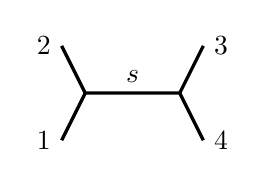
\begin{tikzpicture}[baseline=(current  bounding  box.center), very thick, scale = .3]
\draw (-1,2) node [left] {$2$} -- (0,0) -- node [above] {$s$} (4,0) -- (5,2) node [right] {$3$};
\draw (-1,-2) node [left] {$1$} -- (0,0);
\draw (4,0) -- (5,-2) node [right] {$4$};
\end{tikzpicture} 
= \sum_{\Delta_t\in S} C_{23t}C_{t41} 
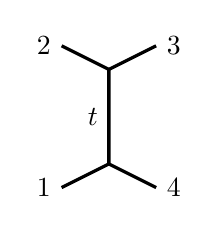
\begin{tikzpicture}[baseline=(current  bounding  box.center), very thick, scale = .3]
 \draw (-2,3) node [left] {$2$} -- (0,2) -- node [left] {$t$} (0,-2) -- (-2, -3) node [left] {$1$};
\draw (0,2) -- (2,3) node [right] {$3$};
\draw (0,-2) -- (2, -3) node [right] {$4$};
\end{tikzpicture}
\ .
\label{csd}
\end{align}
Given the spectrum $S$, crossing symmetry is a system of quadratic equations for the structure constant $C_{\Delta_1,\Delta_2,\Delta_3}$. Requiring that this system has solutions is a strong constraint on the spectrum. 

\begin{defn}[Conformal field theory]
~\label{def:cft}
A (model of) conformal field theory on the Riemann sphere is a spectrum $S$ and a set of correlation functions $\left<\prod_{i=1}^N V_{|w_i\rangle}(z_i)\right>$ with $|w_i\rangle\in S$ that obey all our axioms, in particular crossing symmetry. 
\end{defn}

\begin{defn}[Defining and solving]
 ~\label{def:def}
 To define a conformal field theory is to give principles that uniquely determine its spectrum and correlation functions.
 To solve a conformal field theory is to actually compute them.
\end{defn}

\subsection{Hypergeometric four-point functions}

Crossing symmetry equations typically involve infinite sums, which makes them difficult to solve.
However, if at least one field is degenerate, then the four-point function belongs to the finite-dimensional space of solutions of a BPZ equation. 
For example,
$G(z)= \Big< V_{\langle 2, 1 \rangle}(z) V_{\Delta_1}(0)V_{\Delta_2}(\infty)V_{\Delta_3}(1) \Big>$ is a combination of only two $s$-channel conformal blocks.
These blocks are a particular basis of solutions of the BPZ equation \eqref{eq:ode}, characterized by their asymptotic behaviour near $z=0$ \eqref{eq:gsd}, 
\begin{align}
\mathcal{F}^{(s)}_{\alpha_1-\frac{b}{2}}(z) = z^{b\alpha_1} (1-z)^{b\alpha_3} F(A,B,C,z)\quad , \quad 
 \mathcal{F}^{(s)}_{\alpha_1+\frac{b}{2}}(z) = \left. \mathcal{F}^{(s)}_{\alpha_1-\frac{b}{2}}(z) \right|_{\alpha_1\to Q-\alpha_1} \ ,
\label{gpm}
\end{align}
where $F(A,B,C,z)$ is the hypergeometric function with parameters
\begin{align}
\renewcommand{\arraystretch}{1.3}
\left\{\begin{array}{l}   A = \frac12 + b(\alpha_1+\alpha_3-Q) + b(\alpha_2-\tfrac{Q}{2}) \ , \\
      B = \frac12 + b(\alpha_1+\alpha_3-Q) - b(\alpha_2-\tfrac{Q}{2}) \ , \\
      C = 1 + b(2\alpha_1-Q) \ .
\end{array}\right. 
\label{abc}
\end{align}
Similarly, the two relevant $t$-channel blocks are 
\begin{align}
 \mathcal{F}^{(t)}_{\alpha_3-\frac{b}{2}}(z) &= z^{b\alpha_1} (1-z)^{b\alpha_3} F(A,B,A+B-C+1,1-z)\ ,
 \nonumber \\
 \mathcal{F}^{(t)}_{\alpha_3+\frac{b}{2}}(z) &= \left. \mathcal{F}^{(t)}_{\alpha_3-\frac{b}{2}}(z) \right|_{\alpha_3\to Q-\alpha_3} \ .
\end{align}
Let us build single-valued four-point functions as linear combinations of such blocks. Single-valuedness near $z=0$ forbids terms such as $\mathcal{F}^{(s)}_{\alpha_1-\frac{b}{2}}(z) \mathcal{F}^{(s)}_{\alpha_1+\frac{b}{2}}(\bar z)$, and we must have 
\begin{align}
 G(z) = \sum_{i=\pm} c^{(s)}_{i} \mathcal{F}^{(s)}_{\alpha_1-i\frac{b}{2}}(z) \mathcal{F}^{(s)}_{\alpha_1-i\frac{b}{2}}(\bar z) = \sum_{j=\pm} c^{(t)}_{i} \mathcal{F}^{(t)}_{\alpha_3-j\frac{b}{2}}(z) \mathcal{F}^{(t)}_{\alpha_3-j\frac{b}{2}}(\bar z)\ .
\end{align}
The $s$- and $t$-channel blocks are two bases of the same space of solutions of the BPZ equation, and they are linearly related,
\begin{align}
 \mathcal{F}^{(s)}_{\alpha_1-i\frac{b}{2}}(z) = \sum_{j=\pm} F_{ij} \mathcal{F}^{(t)}_{\alpha_1-j\frac{b}{2}}(z)\ .
\end{align}
In particular, this implies 
\begin{align}
 \frac{c_{+}^{(s)}}{c_{-}^{(s)}} = -\frac{F_{-+}F_{--}}{F_{++}F_{+-}} 
 = \frac{\gamma(A)\gamma(B)\gamma(C-A)\gamma(C-B)}{\gamma(C)\gamma(C-1)}\quad \text{with} \quad \gamma(x) =\frac{\Gamma(x)}{\Gamma(1-x)}\ .
 \label{eq:coc}
\end{align}
We will later express $c_\pm^{(s)}$ in terms of three-point structure constants, and obtain equations for these structure constants.

\section{Liouville theory}

\subsection{Definition}

\begin{defn}[Liouville theory]
 ~\label{def:liou}
 For any value of the central charge $c\in\mathbb{C}$, Liouville theory is the conformal field theory whose spectrum is 
 \begin{align}
  S^\mathrm{Liouville} 
= \int_{\frac{Q}{2}+i\mathbb{R}_+}  d\alpha\ \mathcal V_\alpha \otimes 
   \bar{\mathcal V}_\alpha\ , 
 \end{align}
and whose correlation functions are smooth functions of $b$ and $\alpha$, assuming it exists and its unique.
\end{defn}
Why these values of $\alpha$? If $c\in \mathbb{R}$ we want $\Delta\in\mathbb{R}$ i.e. $\alpha\in \frac{Q}{2}+i\mathbb{R} \cup \mathbb{R}$. But we also want $\Delta$ to be bounded from below, and the natural lower bound is  $\Delta(\alpha=\frac{Q}{2}) =\frac{c-1}{24}$. 

The integral is actually over the half-line $\frac{Q}{2}+i\mathbb{R}_+$ so as not to count representations twice. 
The fields $V_\alpha(z)$ and $V_{Q-\alpha}(z)$ indeed correspond to the same primary state, and we must have a reflection relation, 
\begin{align}
 V_\alpha(z) = R(\alpha) V_{Q-\alpha}(z)\ ,
\end{align}
where the function $R(\alpha)$ is called the reflection coefficient.
Let us schematically write two- and three-point functions in Liouville theory, as well as OPEs:
\begin{align}
 \Big< V_{\alpha_1}V_{\alpha_2} \Big>  &=  \delta(Q-\alpha_1-\alpha_2) + R(\alpha_1)\delta(\alpha_1-\alpha_2)\ ,
 \label{eq:vv}
 \\
 \Big< V_{\alpha_1}V_{\alpha_2}V_{\alpha_3} \Big> & = C_{\alpha_1,\alpha_2,\alpha_3} \quad \text{with} \quad C_{\alpha_1,\alpha_2,\alpha_3} = R(\alpha_1) C_{Q-\alpha_1,\alpha_2,\alpha_3}\ ,
 \\
 V_{\alpha_1}V_{\alpha_2} &= \int_{\frac{Q}{2}+i\mathbb{R}_+} d\alpha\ C_{\alpha_1,\alpha_2,Q-\alpha} \Big( V_\alpha + \cdots\Big)\ .
 \label{eq:v1v2}
\end{align}

In order to have reasonably simple crossing symmetry equations, we need degenerate fields. But the spectrum is made of Verma modules, and the corresponding fields are not degenerate. So we need a special axiom.

\begin{hyp}[Degenerate fields in Liouville theory]
 ~\label{hyp:degl}
 The degenerate fields $V_{\langle 2, 1\rangle}$ and $V_{\langle 1, 2\rangle}$, and their correlation functions, exist. 
\end{hyp}

Let us introduce notations for OPE coefficients of $V_{\langle 2, 1\rangle}$:
\begin{align}
 V_{\langle 2, 1\rangle} V_\alpha \sim C_+(\alpha) V_{\alpha-\frac{b}{2}} + C_-(\alpha)V_{\alpha +\frac{b}{2}}\ .
\end{align}
These OPE coefficients are constrained by the reflection relation, and by the symmetry of $\left< V_{\langle 2, 1\rangle} V_{\alpha_1} V_{\alpha_2}\right>$ under permutations $\alpha_1\leftrightarrow \alpha_2$. 
It can be shown that there exists a field renormalization $V_\alpha(z) \to \lambda(\alpha)V_\alpha(z)$ that preserves the two-point function \eqref{eq:vv}, and is such that
 \begin{align}
  C_+(\alpha) = 1\quad , \quad C_-(\alpha) = \frac{R(\alpha)}{R(\alpha+\frac{b}{2})}\ .
 \end{align}


\subsection{Three-point structure constants}

In Liouville theory, the coefficients $c^{(s)}_\pm$ that appear in hypergeometric four-point functions are 
\begin{align}
 c_{+}^{(s)} = C_+(\alpha_1) C_{\alpha_1-\frac{b}{2},\alpha_2,\alpha_3} 
\quad , \quad 
c_{-}^{(s)}  = C_-(\alpha_1) C_{\alpha_1+\frac{b}{2},\alpha_2,\alpha_3}\ .
\label{cs}
\end{align}
To get an equation for the three-point structure constant $C_{\alpha_1,\alpha_2,\alpha_3}$, we must first determine the  coefficients $C_\pm(\alpha)$. To do this, we consider the special case where the last field is degenerate too, i.e. the four-point function $\Big\langle V_{\langle 2,1 \rangle}(z) V_\alpha(0) V_{Q-\alpha}(\infty) V_{\langle 2,1 \rangle}(1)\Big\rangle$.
In this case, we have
\begin{align}
 c_{+}^{(s)} = C_+(\alpha)C_-(\alpha-\tfrac{b}{2}) = \frac{R(\alpha-\frac{b}{2})}{R(\alpha)} \quad , \quad c_{-}^{(s)} = C_-(\alpha)C_+(\alpha+\tfrac{b}{2}) = \frac{R(\alpha)}{R(\alpha+\frac{b}{2})}\ ,
\end{align}
and eq. \eqref{eq:coc} boils down to 
\begin{align}
 \frac{R(\alpha-\frac{b}{2})R(\alpha+\frac{b}{2})}{R(\alpha)^2} 
 = \frac{\gamma(2b\alpha)\gamma(b(Q-2\alpha))}{\gamma(b(2Q-2\alpha))\gamma(b(2\alpha-Q))}\ .
\end{align}
We could get the same equation with $b\to \frac{1}{b}$ by having $V_{\langle 1,2\rangle}$ instead of $V_{\langle 2,1\rangle}$ in the four-point function. Moreover, we must have $R(\alpha)R(Q-\alpha)=1$. The solution of these equations is
\begin{align}
 R(\alpha) = -b^2  \frac{\gamma(b(2\alpha-Q))}{\gamma(\frac{1}{b}(Q-2\alpha))}\ .
\end{align}
This also determines $C_\pm(\alpha)$, and we can deduce a shift equation for three-point structure constants from eq. \eqref{eq:coc} and \eqref{cs},
\begin{align}
 \frac{C_{\alpha_1+b,\alpha_2,\alpha_3}}{C_{\alpha_1,\alpha_2,\alpha_3}} = b^{-4}\frac{\gamma(2b\alpha_1)\gamma(2b\alpha_1+b^2)}{\prod_{\pm,\pm} \gamma\left(b\alpha_1\pm b(\alpha_2-\frac{Q}{2})\pm b(\alpha_3-\frac{Q}{2})\right)}\ .
\label{fcc}
\end{align}
Again, the equation with $b\to \frac{1}{b}$ should hold too. In order to solve these equations, we need a function that produces Gamma functions when its argument is shifted by $b$ or $\frac{1}{b}$. 

\begin{defn}[Upsilon function]
~\label{def:upsilon}
 For $b>0$, let $\Upsilon_b(x)$ be the unique (up to a constant factor) holomorphic function that obeys the shift equations
 \begin{align}
  \frac{\Upsilon_b(x+b)}{\Upsilon_b(x)} = b^{1-2bx} \gamma(bx)\qquad \text{and} \qquad \frac{\Upsilon_b(x+\frac{1}{b})}{\Upsilon_b(x)} = b^{\frac{2x}{b}-1} \gamma(\tfrac{x}{b})\ .
\label{upup}
\end{align}
For $ib>0$, the meromorphic function 
\begin{align}
 \hat{\Upsilon}_b(x) = \frac{1}{\Upsilon_{ib}(-ix+ib)}\ ,
\end{align}
then obeys the same shift equations.
\end{defn}
The functions $\Upsilon_b(x)$ and $\hat\Upsilon_b(x)$ can respectively be defined for $\Re b>0$ and $\Re ib>0$ by analytic continuation. And we have 
\begin{align}
 \Upsilon_b(x) = \prod_{m,n=0}^\infty f\left(\frac{\frac{Q}{2}-x}{\frac{Q}{2}+mb+nb^{-1}}\right) \quad \text{with} \quad f(x)=(1-x^2)e^{x^2}\ .
\end{align}
Using the functions $\Upsilon_b(x)$, we can write a solution $C$ of the shift equations \eqref{fcc} for three-point structure constants,
\begin{align}
 C_{\alpha_1,\alpha_2,\alpha_3} =  \frac{ \Upsilon_b(2\alpha_1) \Upsilon_b(2\alpha_2) \Upsilon_b(2\alpha_3)}{\Upsilon_b(\alpha_1+\alpha_2+\alpha_3-Q) \Upsilon_b(\alpha_1+\alpha_2-\alpha_3)\Upsilon_b(\alpha_2+\alpha_3-\alpha_1)\Upsilon_b(\alpha_3+\alpha_1-\alpha_2)} \ .
\label{caaa}
\end{align}
This solution is called the DOZZ formula for Dorn, Otto, A.
Zamolodchikov and Al. Zamolodchikov. It holds if
$c\notin ]-\infty, 1]$ i.e. $b\notin i\mathbb{R}$. 
On the other hand, doing the replacement $\Upsilon_b\to \hat\Upsilon_b$, we obtain a solution $\hat C$ that holds if  $c\notin [25,\infty[$ i.e. $b\notin \mathbb{R}$.

The solution is unique if $b$ and $b^{-1}$ are aligned, i.e. if $b^2\in\mathbb{R}$:
\begin{equation}
 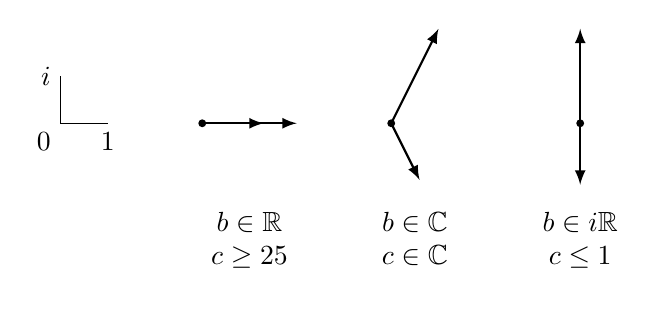
\begin{tikzpicture}[baseline=(current  bounding  box.center), scale = .6]
\draw (0, 2) node[left]{$i$} -- (0, 1) node[below left] {$0$} -- (1, 1) node[below] {$1$};
\draw [thick, latex-latex] (11,3) -- (11,1) node[fill, circle, minimum size = 1mm, inner sep = 0]{} -- (11,-.3);
\draw [thick, latex-latex] (8,3) -- (7,1) node[fill, circle, minimum size = 1mm, inner sep = 0]{}-- (7.6,-.2);
\draw [thick, latex-latex] (5,1) -- (3,1) node[fill, circle, minimum size = 1mm, inner sep = 0]{} -- (4.3,1) ;
\node at (4, -1.5){$\begin{array}{c} b\in \mathbb{R} \\ c\geq 25 \end{array}$};
\node at (7.5, -1.5){$\begin{array}{c} b\in \mathbb{C} \\ c\in\mathbb{C} \end{array}$};
\node at (11, -1.5){$\begin{array}{c} b\in i\mathbb{R} \\ c\leq 1 \end{array}$};
 \end{tikzpicture}
\end{equation}
However, for general values of $c$, both $C$ and $\hat C$ are solutions, and there are actually infinitely many other solutions. In order to prove the existence and uniqueness of Liouville theory, we have to determine which solutions lead to crossing-symmetric four-point functions.


\subsection{Four-point functions}

The $s$-channel decomposition of a Liouville four-point function reads 
\begin{align}
 \Big< V_{\alpha_1}(z) V_{\alpha_2}(0) V_{\alpha_3}(\infty) V_{\alpha_4}(1)\Big> = \frac12 \int_{\frac{Q}{2}+i\mathbb{R}} d\alpha\ C_{\alpha_1,\alpha_2,Q-\alpha} C_{\alpha,\alpha_3, \alpha_4} \mathcal{F}_{\alpha}^{(s)}(z) \mathcal{F}_{\alpha}^{(s)}(\bar z)\ ,
 \label{eq:ccff}
\end{align}
where the structure can be $C$ or $\hat C$. Let us accept that the conformal blocks $\mathcal{F}_{\alpha}^{(s)}(z)$ have poles when $\alpha = \alpha_{\langle r, s\rangle} $ \eqref{eq:ars}, the momentums for which the $s$-channel representation becomes reducible.
We now plot the positions of these poles (blue regions) relative to the integration line (red), depending on the central charge:
\begin{align}
 \newcommand{\polewedge}[3]{
\begin{scope}[#1]
\node[blue, draw,circle,inner sep=1pt,fill] at (0, 0) {};
\node[#3] at (0,0) {#2};
\filldraw[opacity = .1, blue] (0,0) -- (4, -4) -- (4, 4) -- cycle;
\end{scope}
}
\begin{array}{ccc}
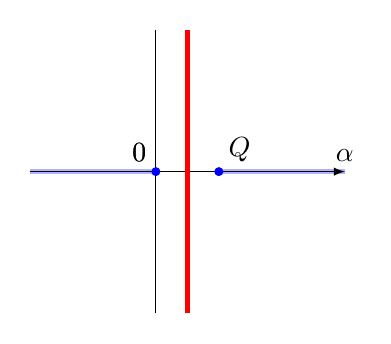
\begin{tikzpicture}[scale = .4, baseline=(current  bounding  box.center)]
 \draw[ultra thick, blue, opacity = .3] (0,0) -- (-4,0);
 \draw[ultra thick, blue, opacity = .3] (2,0) -- (6,0);
  \draw[-latex] (-4,0) -- (0, 0) node[above left] {$0$} -- (6,0) node [above] {$\alpha$};
  \draw (0, -4.5) -- (0, 4.5);
  \draw[ultra thick, red] (1, -4.5) -- (1, 4.5);
  \node[blue, draw,circle,inner sep=1pt,fill] at (0, 0) {};
\node[above left] at (0,0) {$0$};
\node[blue, draw,circle,inner sep=1pt,fill] at (2, 0) {};
\node[above right] at (2,0) {$Q$};
 \end{tikzpicture}
 & 
 \begin{tikzpicture}[scale = .4, baseline=(current  bounding  box.center)]
  \draw[-latex] (-4,0) -- (0, 0) node[above left] {$0$} -- (6,0) node [above] {$\alpha$};
  \draw (0, -4.5) -- (0, 4.5);
  \draw[ultra thick, red] (1, -4.5) -- (1, 4.5);
  \polewedge{rotate = 180}{$0$}{above left};
  \polewedge{shift = {(2, .3)}}{$Q$}{above right};
 \end{tikzpicture}
 &
 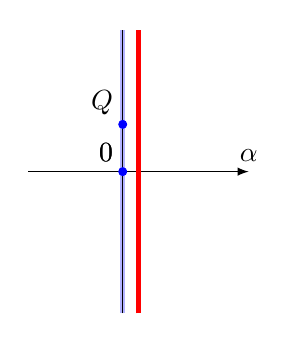
\begin{tikzpicture}[scale = .4, baseline=(current  bounding  box.center)]
  \draw[-latex] (-3,0) -- (0, 0) node[above left] {$0$} -- (4,0) node [above] {$\alpha$};
  \draw[ultra thick, blue, opacity = .3] (0, -4.5) -- (0, 4.5);
  \draw (0, -4.5) -- (0, 4.5);
  \draw[ultra thick, red] (.5, -4.5) -- (.5, 4.5);
  \node[blue, draw,circle,inner sep=1pt,fill] at (0, 0) {};
\node[above left] at (0,0) {$0$};
\node[blue, draw,circle,inner sep=1pt,fill] at (0, 1.5) {};
\node[above left] at (0,1.5) {$Q$};
 \end{tikzpicture}
 \vspace{3mm}
 \\
 c\geq 25 & c\text{ generic}  &  c\leq 1
\end{array}
\end{align}
The four-point function built from $C$ is analytic on $c\notin ]-\infty,1]$. So if Liouville theory exists for $c\geq 25$, then it also exists for $c$ generic, with the same structure constant $C$. 
On the other hand, the limit $c\to ]-\infty, 1]$ is singular. Actually, for $c\leq 1$, the integration line has to be slightly shifted in order to avoid the poles. So the structure constant $\hat C$ is expected to be valid only for $c\leq 1$.

That is how far we can easily get with analytic considerations. 
Numerical tests of crossing symmetry confirm that Liouville theory exists for all values of $c$, with the three-point structure constants $\hat C$ if $c\leq 1$, and $C$ otherwise \cite{rs15}.

Raoul Santachiara will talk about the application of Liouville theory to Random Energy Models. For this application we need to determine the behaviour of four-point functions in the limit $z\to 0$ for $c\geq 25$. This is a priori dominated by the state with the lowest conformal dimension $\Delta(\alpha=\frac{Q}{2})$. At this point each structure constants in eq. \eqref{eq:ccff} has a simple zero, and 
\begin{align}
 \Big< V_{\alpha_1}(z) V_{\alpha_2}(0) V_{\alpha_3}(\infty) V_{\alpha_4}(1)\Big>  & \underset{z\to 0}{\sim} \int_{\frac{Q}{2}+i\mathbb{R}} d\alpha\ (\alpha-\tfrac{Q}{2})^2 |z|^{2\Delta(\alpha)-2\Delta(\alpha_1)-2\Delta(\alpha_2)} \ ,
 \\
& \sim \frac{ |z|^{2\Delta(\frac{Q}{2})-2\Delta(\alpha_1)-2\Delta(\alpha_2)} }{ |\log |z||^\frac32 }\ .
\end{align}
This however assumes that the four fields $V_{\alpha_i}$ belong to the spectrum, i.e. $\alpha_i\in\frac{Q}{2}+i\mathbb{R}$.
For other values of $\alpha_i$, we can encounter poles of the structure constants.  Such poles can cancel the zeros of the structure constants, in which case the exponent of $\log|z|$ becomes $\frac12$ instead of $\frac32$. 
It can also happen that poles give rise to discrete terms in the OPE in addition to the continuum. If the four-point function is dominated by such a discrete term, then we lose the logarithmic factor altogether.

% \section*{Acknowledgements}

\bibliographystyle{cft}
\bibliography{cft}


\end{document}

